% -*- root: ../../main.tex -*-
\section{Audio Manager}
\label{sec:audio_manager_design}
I videogiochi richiedono in generale il lancio di un elevato numero di \textbf{suoni} per partita.
Questi suoni rientrano generalmente in una delle seguenti categorie:
\begin{itemize}
    \item \textbf{Effetti sonori:} sono generalmente legati a \textbf{eventi} o a \textbf{interazioni} con la \textbf{GUI} del gioco.
    \item \textbf{Musica:} ricoprono un ruolo di \textbf{sottofondo} e vengono riprodotto con \textbf{minor frequenza}.
\end{itemize}

\paragraph{Un modello ad agenti:}
L'elevata frequenza di eventi ha portato allo sviluppo di un \textbf{Agente} al quale è stato affidato il compito di \textbf{gestire} e \textbf{manipolare} internamente tutti gli aspetti sonori del gioco.

Il \texttt{SoundAgent} è caratterizzato da un  \textbf{flusso di controllo separato} e utilizza una \textbf{coda di eventi} per tracciare tutte le \textbf{azioni} che deve effettuare. Gli utilizzatori possono infatti \textbf{accodare eventi} esternamente \textbf{senza} così \textbf{inquinare} l'operatività del \textbf{proprio flusso} di controllo.
Un flusso di controllo separato consente di \textbf{disaccoppiare} al massimo il carico di lavoro, permettendo così di non gravare sulla logica principale del programma né tantomeno sulla \textbf{View}.

\begin{figure}[H]
	\centering
	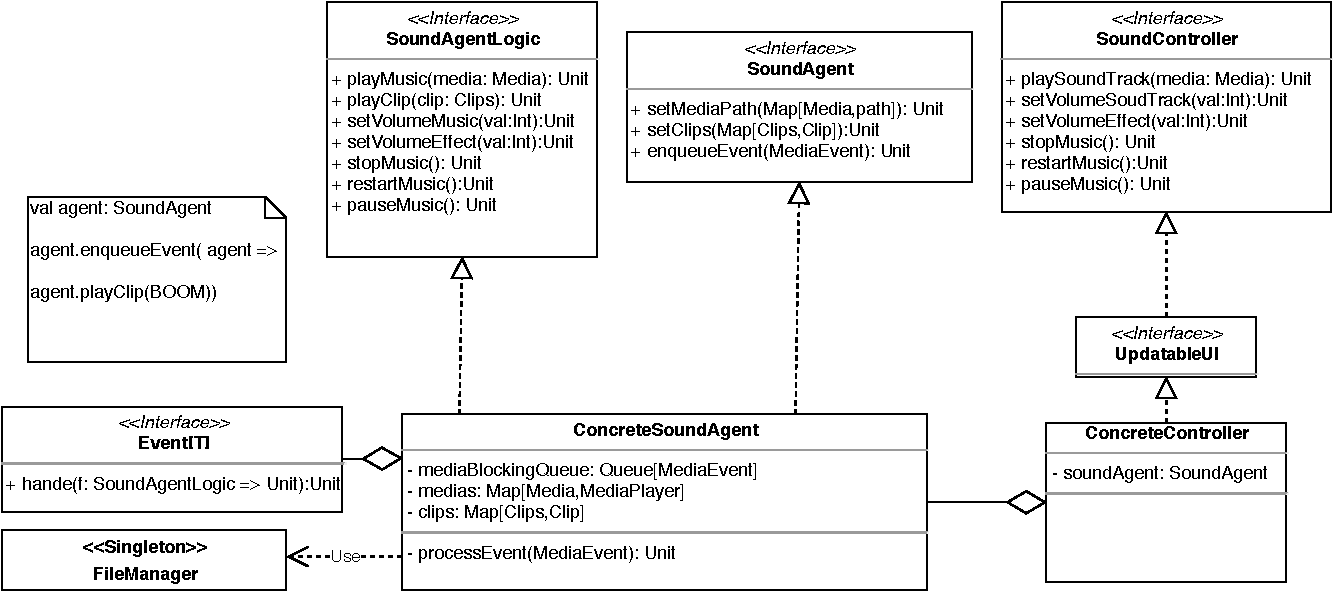
\includegraphics[width=0.99\columnwidth]{drawio/audioAgent/audioAgent.pdf}
	\caption{Diagramma di classe rappresentante la struttura del SoundAgent.}
	\label{fig:AudioAgent}
\end{figure}

Un solo \texttt{SoundAgent} è in grado di riprodurre una grossa \textbf{quantità di clip}, ciò nonostante è possibile istanziarne più di uno, questo per non limitare il numero di suoni. È inoltre possibile creare \texttt{SoundAgent} specifici.

Un eventuale utilizzatore potrà quindi schedulare un nuovo evento semplicemente sfruttando il pattern \textbf{Strategy} implementando l'interfaccia funzionale \texttt{SoundAgentLogic}.
Questo consente di evitare l'utilizzo reiterato di \textbf{match case} all'interno dell'agente, rendendo l'esecuzione più \textbf{performante} e il \textbf{codice più snello}.